\chapter{Neural Net based Electronics Response Modeling}
\label{chap:elect_resp}

\section{Introduction}
As discussed in chapter \ref{chap:detectors}, HPGe detectors provide excellent energy resolution and good pulse-shape–based event identification, making them critical for low-background physics searches such as neutrinoless double-beta decay $0\nu\beta\beta$. However, the signal from HPGe detector must pass through an electronic readout chain consisting of components such as preamplifier, filtering stages, and digitization. These electronics transform the signal in ways that can distort pulse shapes, alter the rise time, and add overshoots/undershoots or baseline shifts. Accurately modeling this transformation is crucial for producing realistic pulse-shape simulations.

This chapter begins with an overview of typical HPGe detector readout electronics. It is followed by an overview of {\Ltwo}  electronics and how electronics introduce distortions in waveforms, called electronics response. This is followed by challenges in modeling the electronics response and a neural network approach to it.

\section{{\Ltwo} readout electronics}

{\Ltwo} uses a resistive-feedback charge-sensitive amplifier (CSA) to minimize noise and achieve low radioactive background. The first stage is referred to as the Low-Mass Front End (LMFE). LMFE is placed inside the experiment’s liquid argon cryostat, only a few millimeters from the point contact of each HPGe detector \cite{Willers_2020}. LMFE is thus constructed with high radio-pure materials with tolerance typically on the order of $1\mu$ Bq per channel. LMFE builds upon one developed by {\MJD} and is produced using Suprasil substrates, titanium-gold (TiAu) traces, an in-die junction field effect transistor (JFET, Moxtek MX11), and thin-film amorphous germanium feedback resistors that can operate at cryogenic temperatures. 

\begin{figure}[!htb]%[htb!]
  %[trim={left bottom right top},clip]
    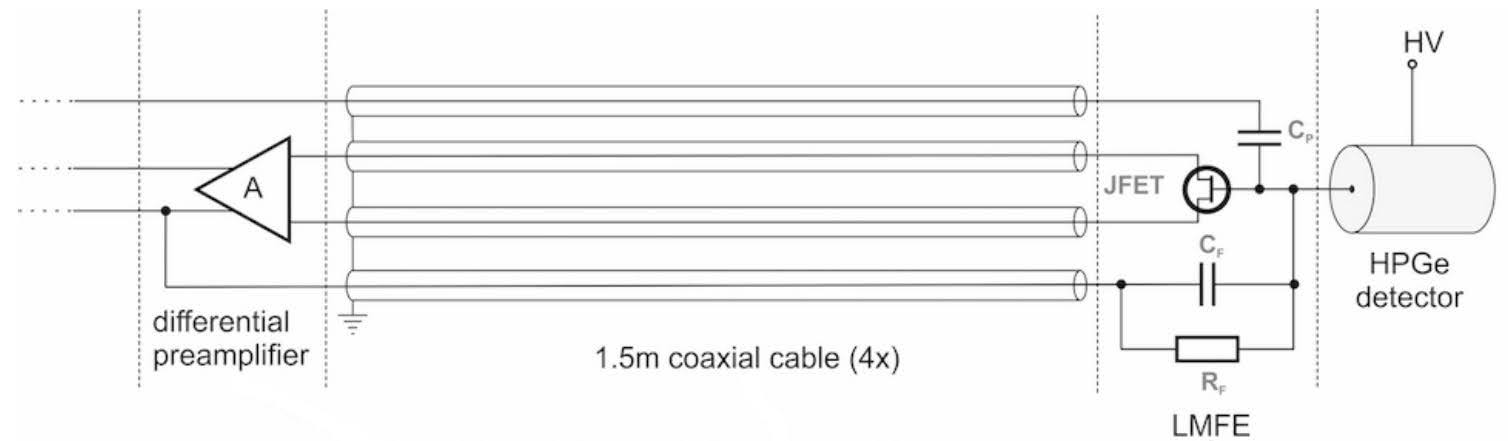
\includegraphics[width=0.99\linewidth,trim={1pc 0pc 1pc 0pc},clip]{ch5/figs/l200_elec_diagram.jpg}
    \caption{A Schematic of the Demonstrator signal readout chain.\cite{Willers_2020}}
   \label{fig:l200_elec_model}
\end{figure}

\begin{figure}[!htb]%[htb!]
  %[trim={left bottom right top},clip]
  \centering
    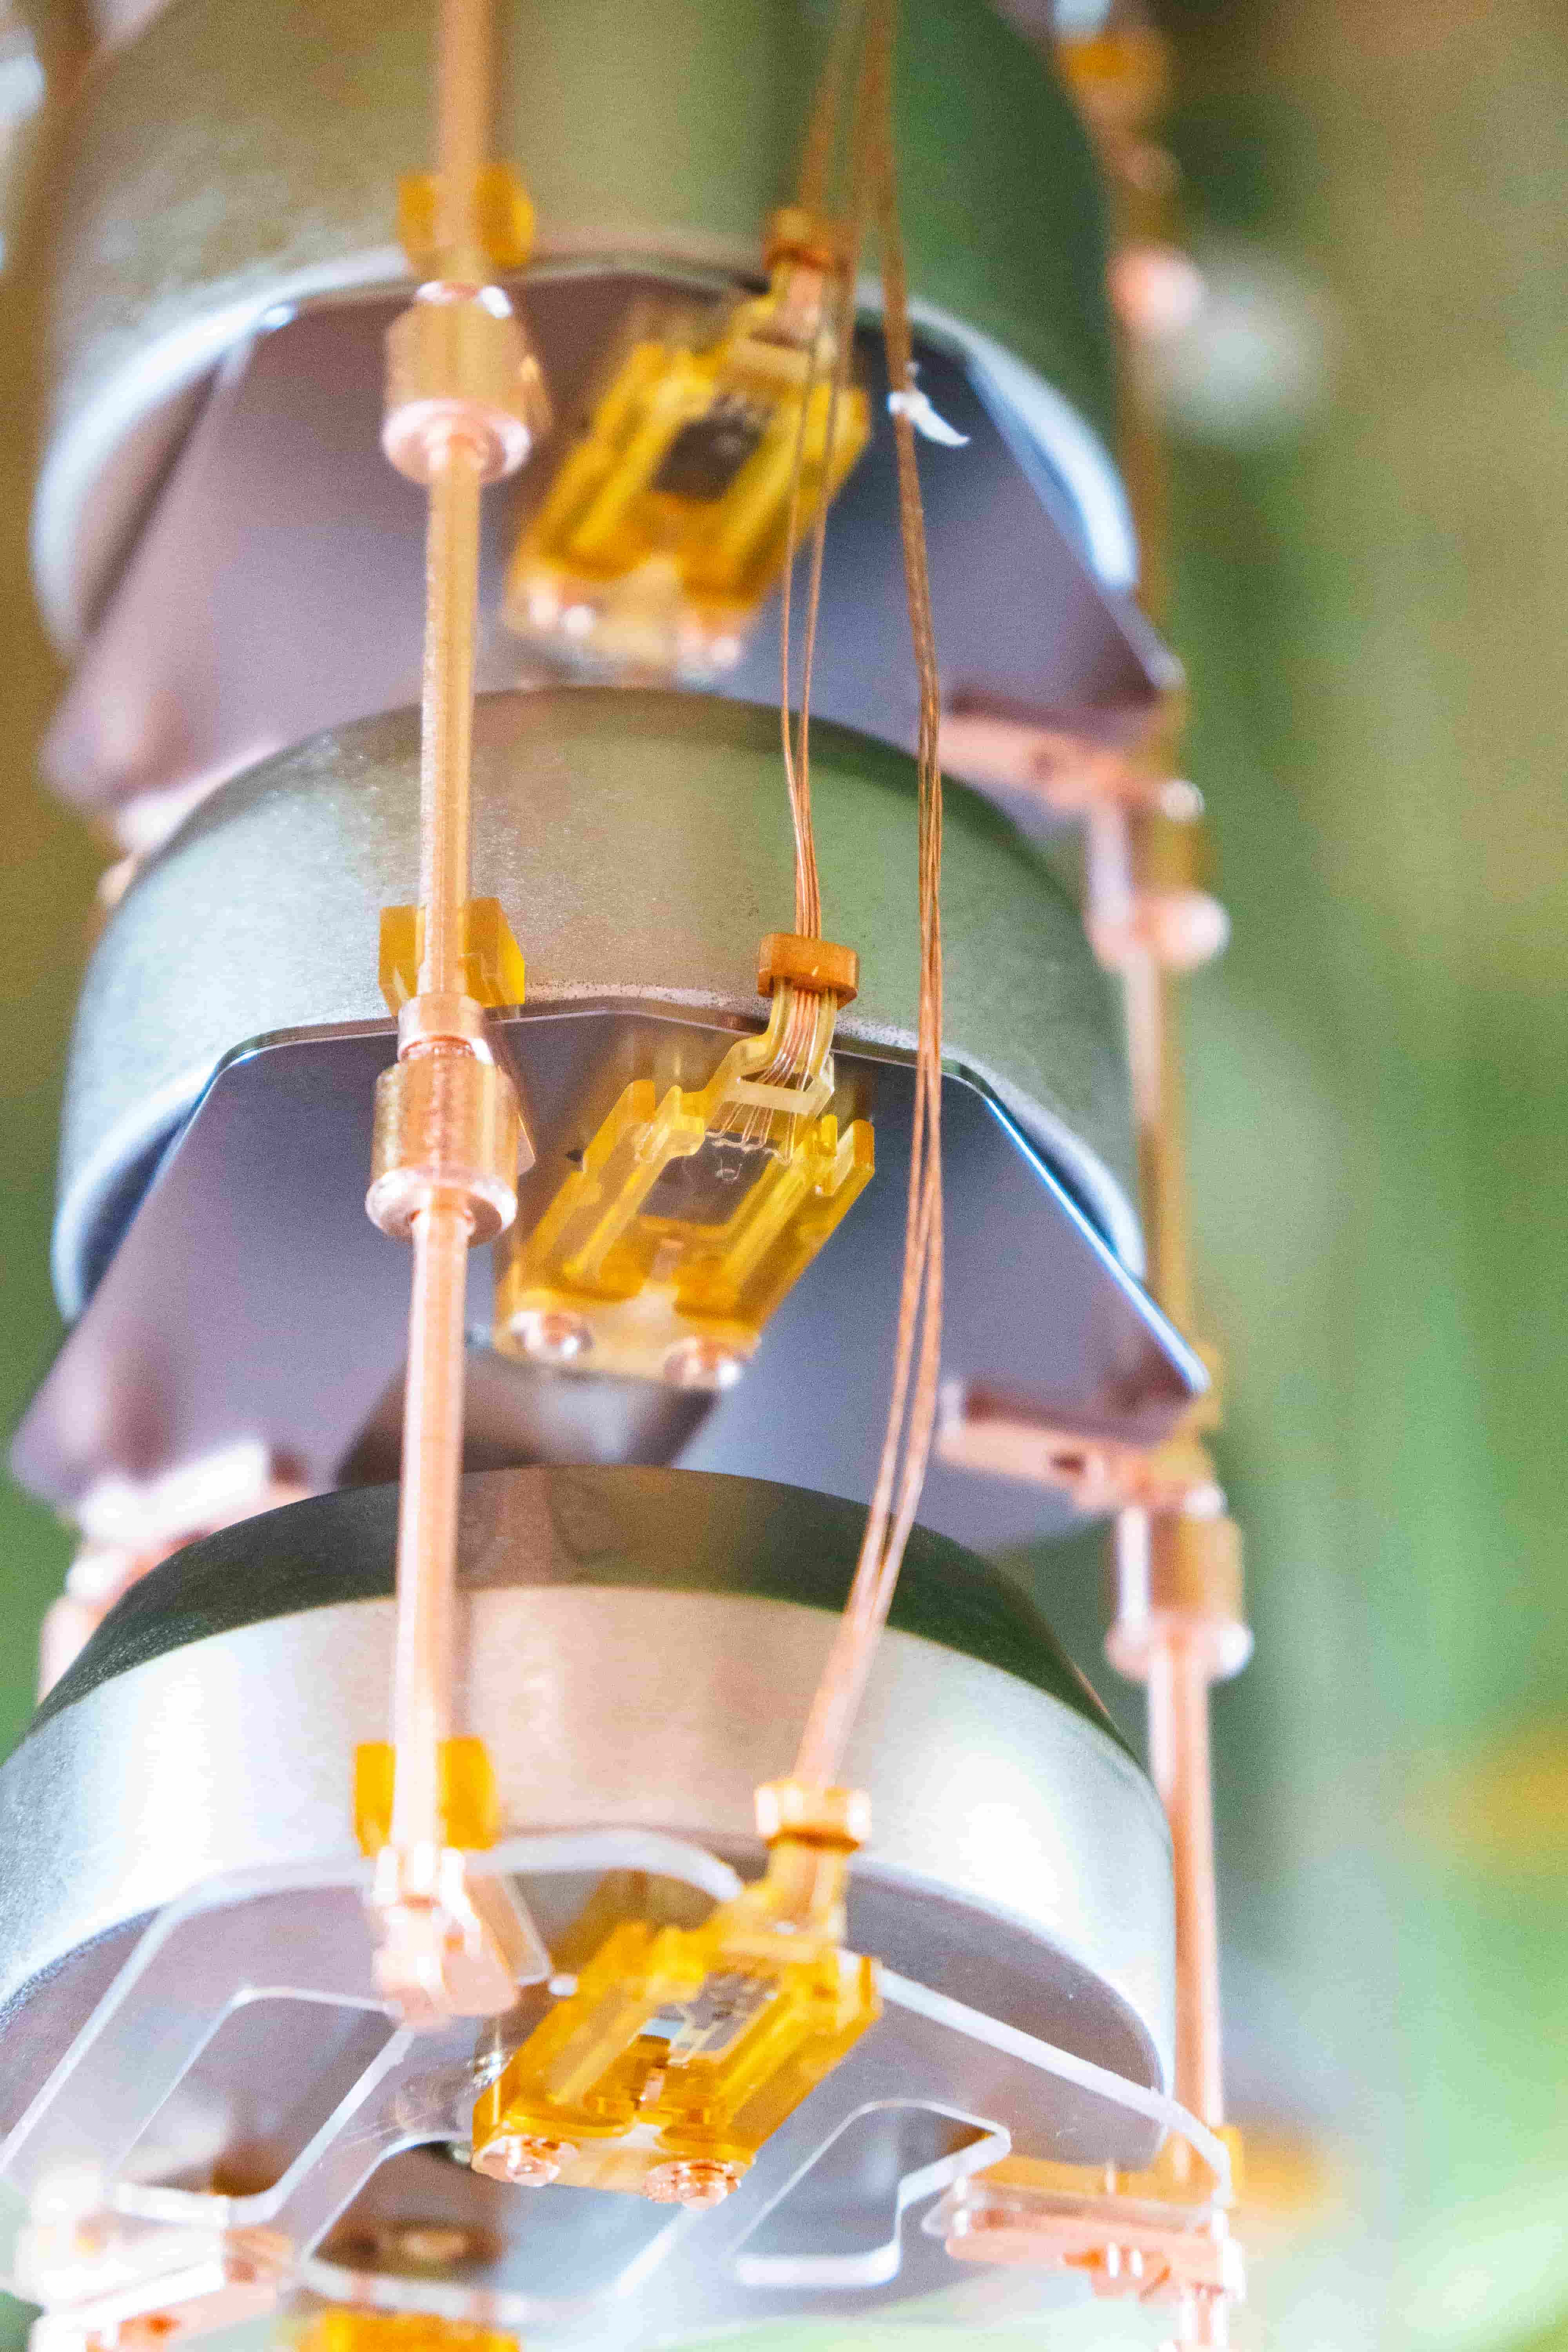
\includegraphics[width=0.32\linewidth,trim={1pc 0pc 1pc 0pc},clip]{ch5/figs/l200_det_close_up.jpg}
    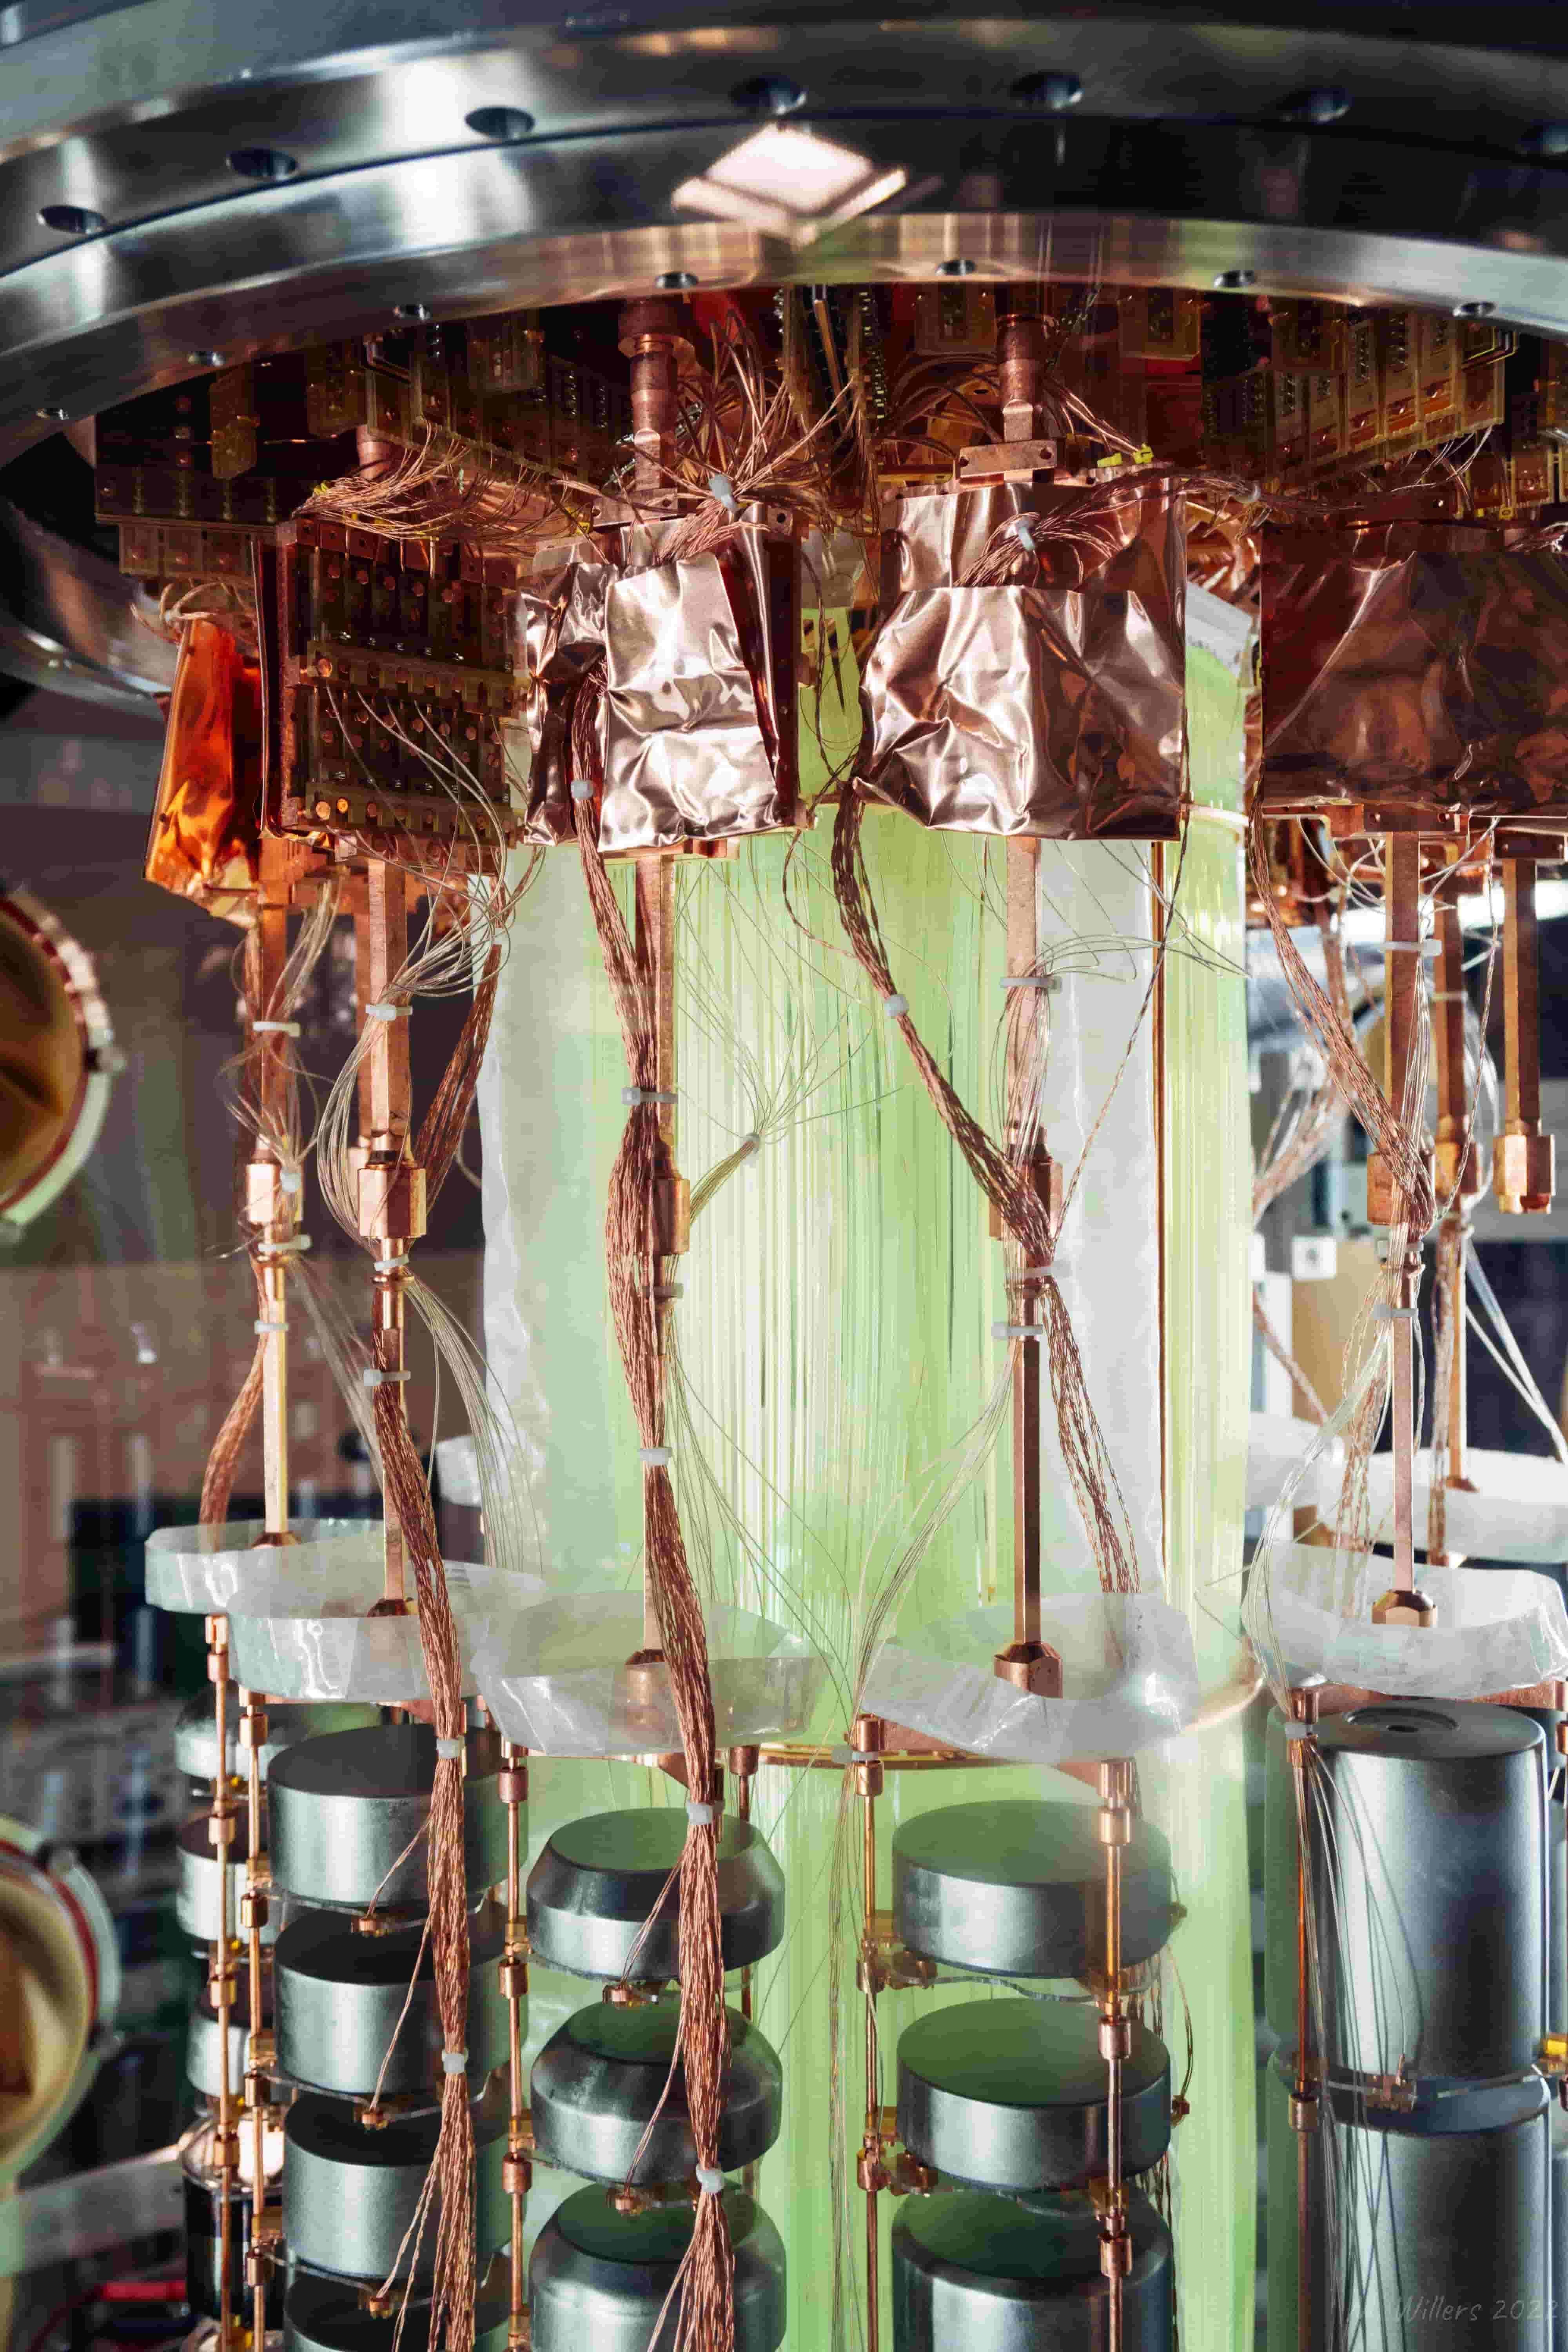
\includegraphics[width=0.32\linewidth,trim={1pc 0pc 1pc 0pc},clip]{ch5/figs/l200_elec_picture.jpg}
    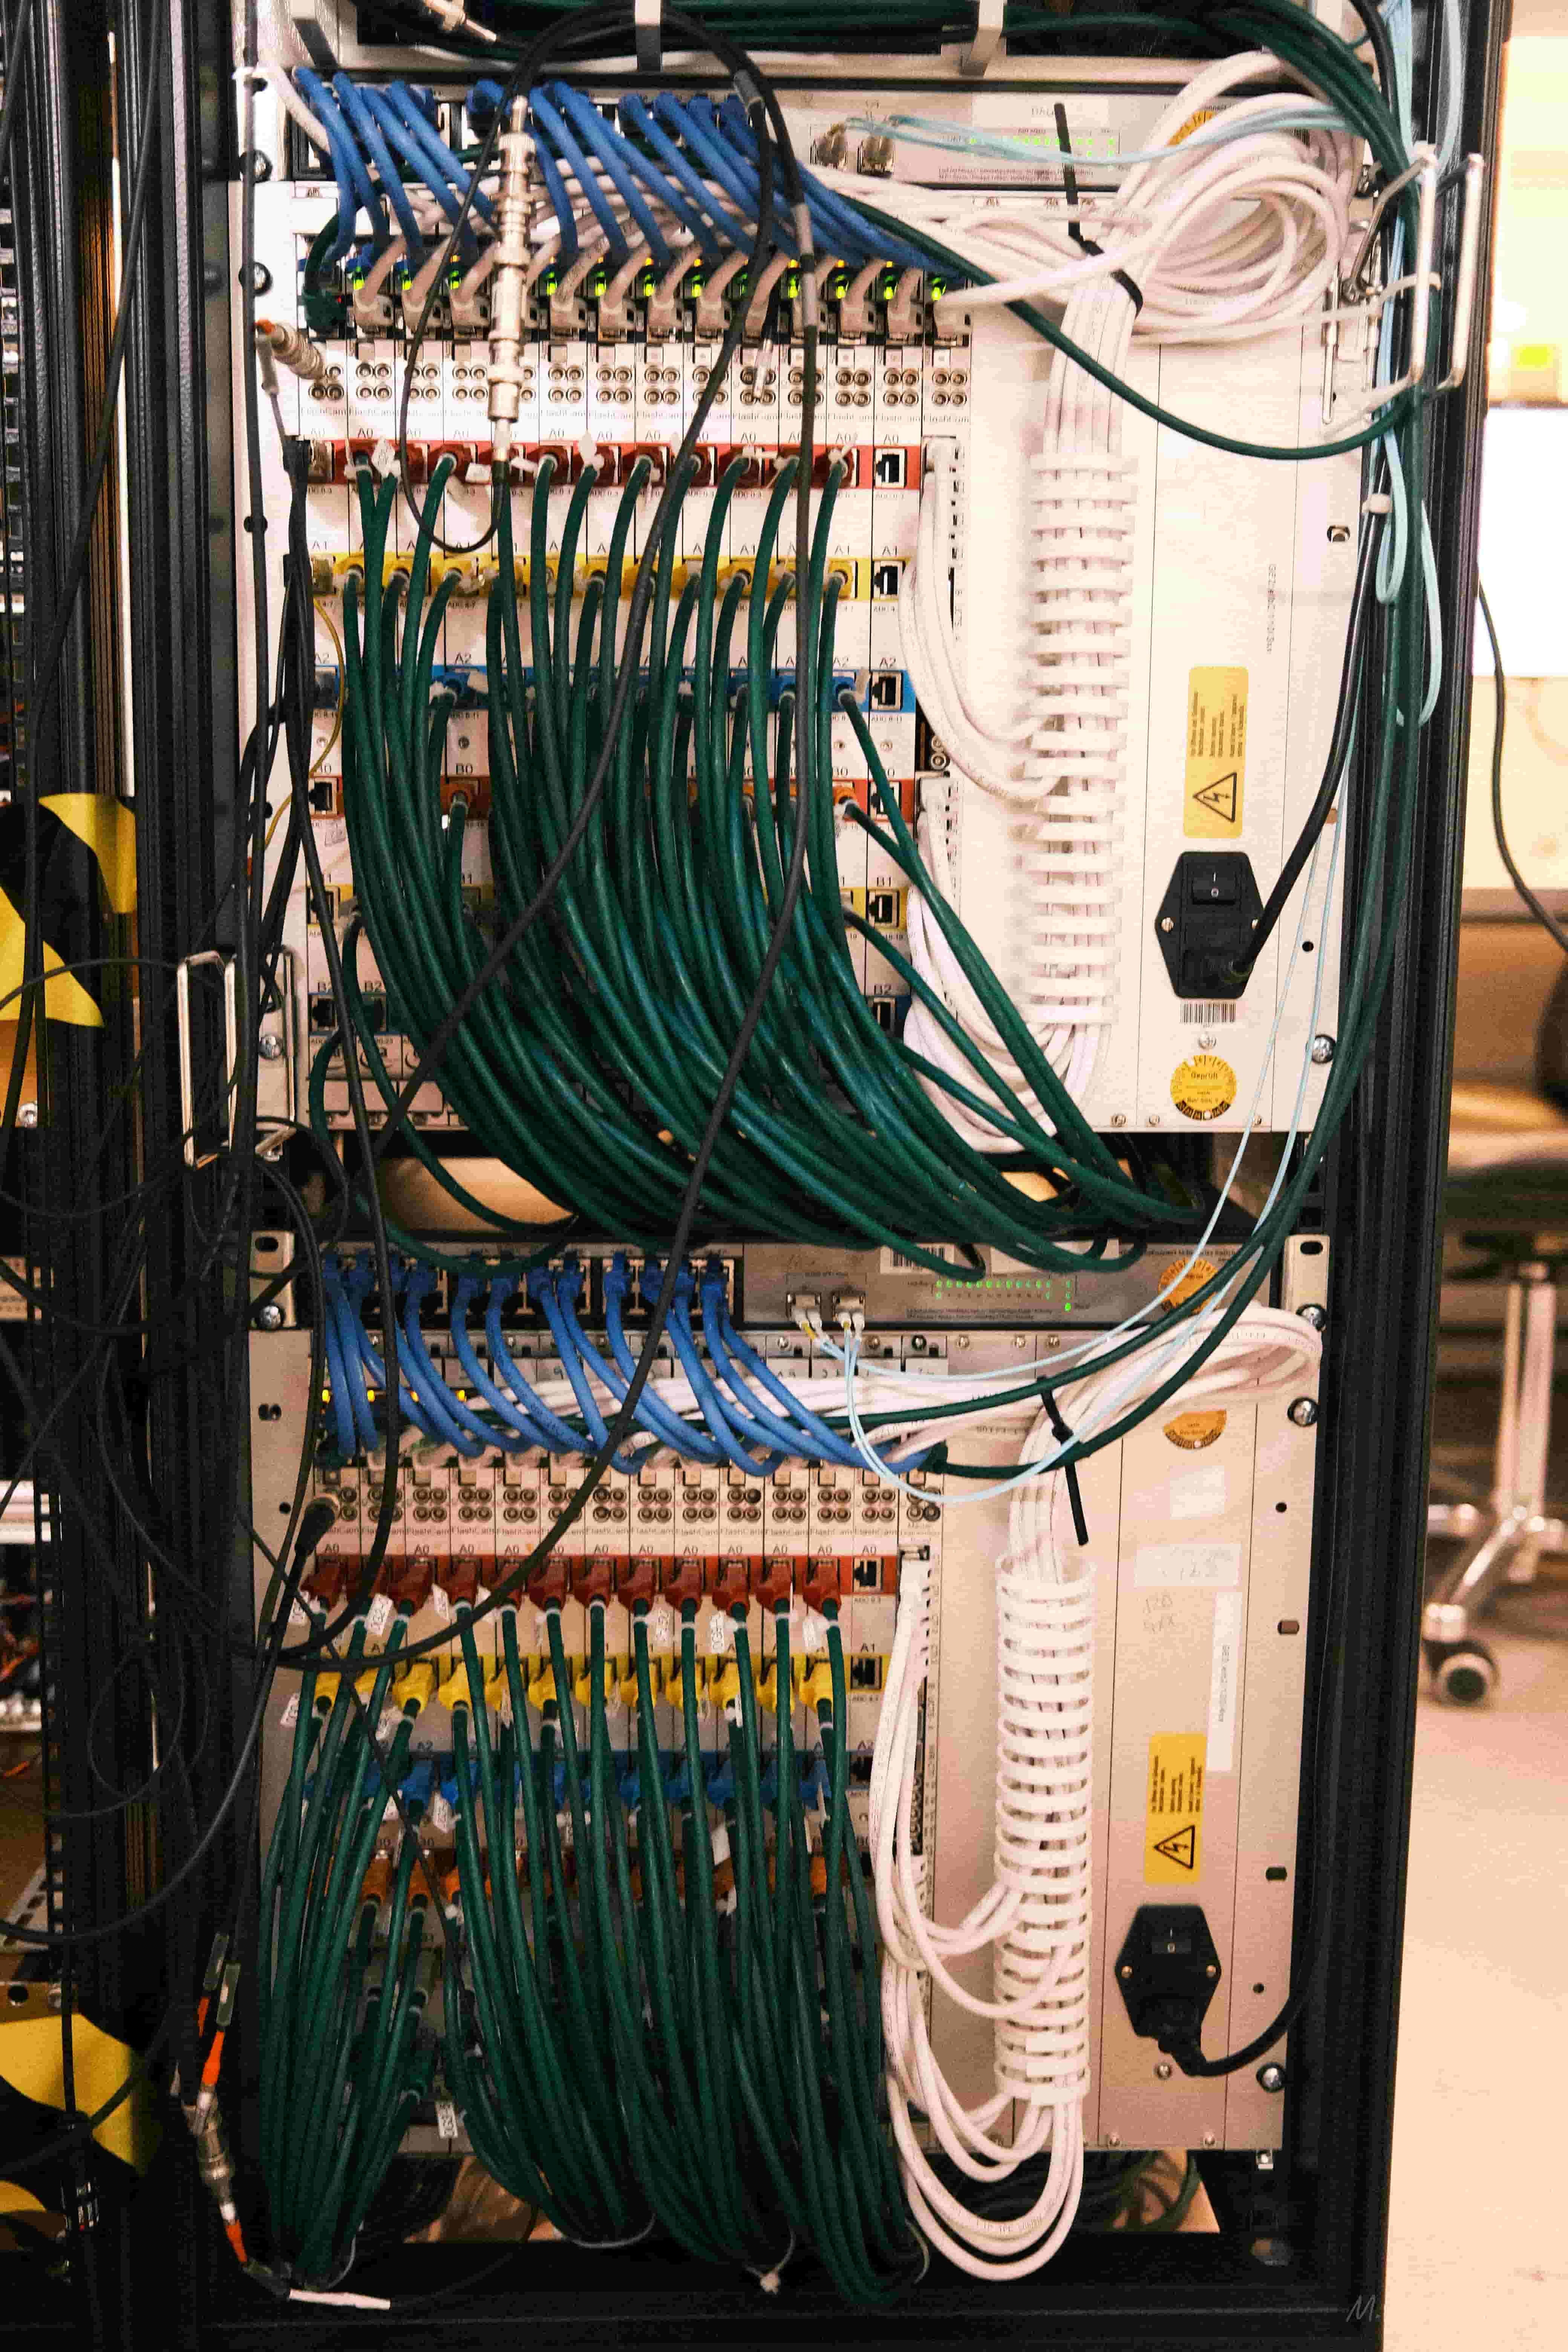
\includegraphics[width=0.32\linewidth,trim={1pc 0pc 1pc 0pc},clip]{ch5/figs/l200_flashcam_crate.jpg}
    \caption{Picture of the front end electronics of {\Ltwo}. Left show close up of the detector with the LMFE, middle shows the detector strings front end electronics and right shoes the Flashcam crates in the DAQ rack. Photo: Michael Willers}
   \label{fig:l200_elec}
\end{figure}



The second amplifier is based on a folded cascode arrangement and located $30$–$150$ cm from the detector to provide additional gain and to convert the signal to a differential output. This stage can tolerate slightly higher radioactivity levels of $50\mu$ Bq per channel and is built using screened commercial surface-mount components on Kapton circuit boards called the CC4. The second stage is connected to the the data acquisition system using a $\thicksim 10$ m long transmission line. An active buffer called Head Electronics receives the signals from the second stage. This adjusts offsets and gain while providing impedance matching. Finally the signals is fed into a FlashCam where the signal is digitized and stored for analysis.

Together these design choices enable sub 3keV FWHM energy resolution in the ROI at $Q_{\beta\beta}$ 2039 keV while contributing minimally to the overall radioactive background. They also enable a fast rise time of $\thicksim 0.100$ ns which allows pulse shape discrimination of the signals. Additionally, they have a high range of up to 10 MeV that enables measuring high-energy alpha decays which would provide additional information for background modelling.

\section{Electronics Influence on Waveforms}

Despite careful design and component selection, the LEGEND-200 electronics chain inevitably modifies the detector’s raw current signals. Figure~\ref{fig:sim_data_comp} shows some of these effects by comparing a simulated waveform (blue) with a corresponding real data pulse (red).

The baseline is the region before $t_0$, the start of the wavefrom. Ideally, this baseline should remain near a stable DC offset determined by the preamplifier’s quiescent operating point. Two factors can shift or tilt the baseline. First, a slow high-pass filter effect (on the order of milliseconds) arises from the capacitive coupling between the first and second preamplifier stages. Second, if events occur in rapid succession, the tail from one pulse may not fully decay before the next arrives, causing the baseline to drift or undershoot. These shifts become especially noticeable at higher rates, leading to soft pile-up where partial overlap deforms the apparent starting level of subsequent pulses. 

The rising edge, shown in orange region, is the most visible part of the waveform resulting from movement of electrons and holes from the energy deposition. The long cable runs and folded-cascode amplifier stages introduce a finite bandwidth, effectively acting as a low-pass filter that damps the highest-frequency components. As a result, the observed rising edge in real data tends to be broader and smoother than in simulations. 

The RC decay tail (light blue region) arises from the CSA feedback network in the LMFE, where the detector current is integrated on a feedback capacitor and slowly discharged by the feedback resistor. The second stage of amplification often has a shorter differentiator-like time constant, further modifying the decay shape seen in data. Taken together, these processes create a voltage pulse with a multi-exponential decay. 

Overall, the three waveform regions, baseline, rising edge, and tail, are each influenced by different parts of the LEGEND-200 electronics chain. Circuit simulations such as SPICE can reproduce some of the bulk features but minute responses such as parasitic inductance, JFET nonlinearity, or thermal drifts are hard to model.

\begin{figure}[!htb]%[htb!]
  %[trim={left bottom right top},clip]
    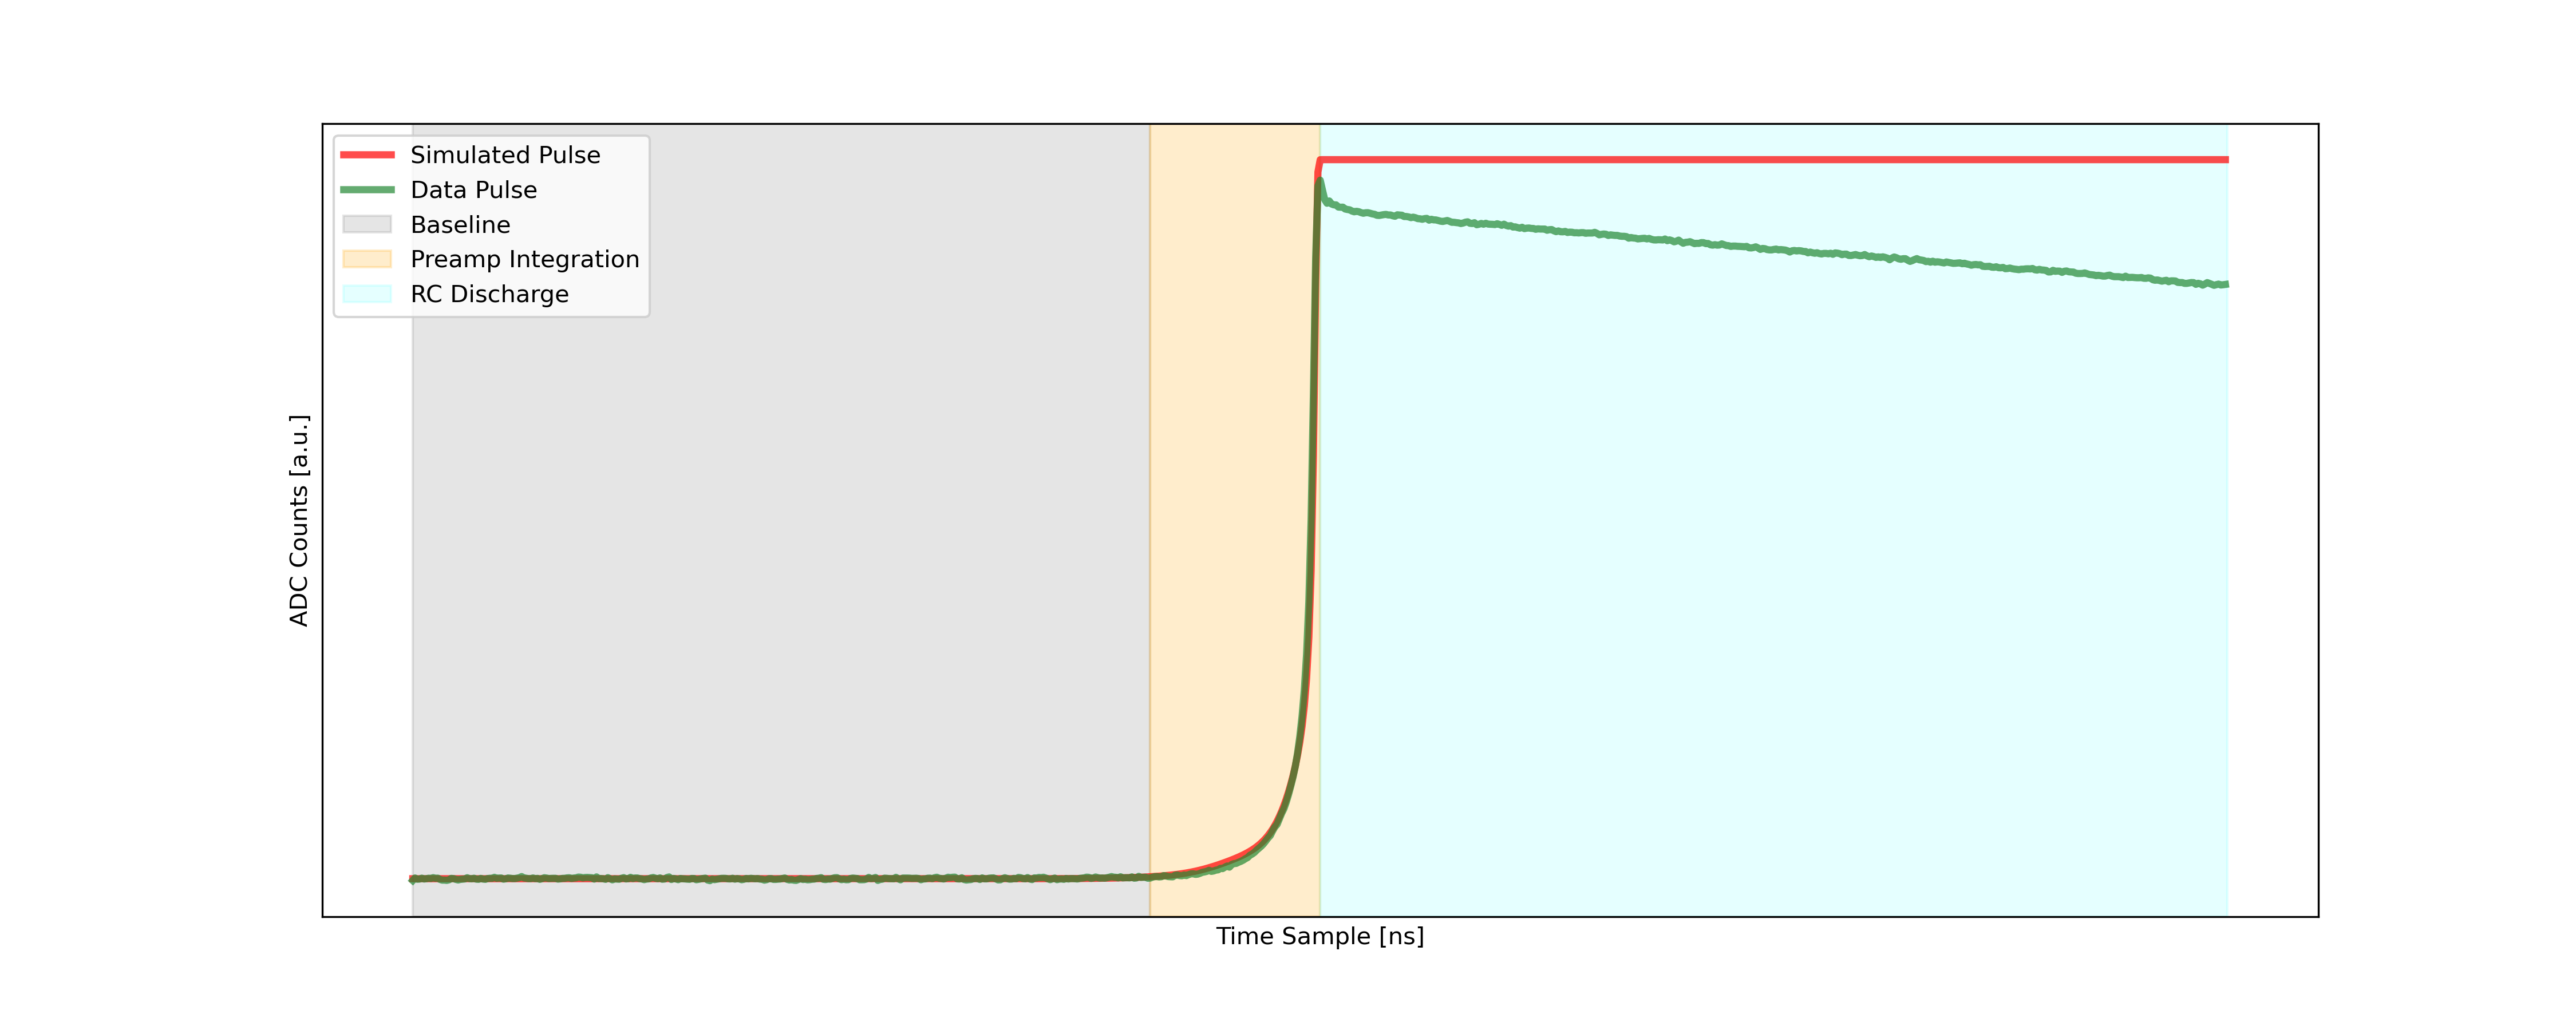
\includegraphics[width=\linewidth,trim={4cm 0pc 3.5cm 0pc},clip]{ch5/figs/wf_comp_sim_data.png}
    \caption{Comparison of a simulated waveform with a real data pulse.}
    \label{fig:sim_data_comp}
\end{figure}

\section{Challenges in Modeling Electronics Response}


Pulse shape simulation aims at generating pulses that are similar to the actual detector pulses. This allows to create a ground-truth datasets where a direct mapping can be established between a simulated pulse and its corresponding incident particle. This would enable applying the same cuts to the simulations as data and precisely calculate their efficiency. Suppose we apply an existing pulse shape discrimination cut~\cite{AvsE} to this dataset. In that case, it will be immediately apparent which event topologies lead to the signal sacrifice or background contamination of this cut. This information will be pivotal for the evaluation and further improvement of cut efficiency. 

% In point-contact-style detectors, the signal is read out at a small point-like ground electrode, with the resulting electric field leading to sharply rising detector pulses. This readout electrode is instrumented with an amplification and digitization chain. 


As discussed in previous section frequency-dependent response function must then be added to the simulations to reproduce the detector response. The electronic transfer function describes the series of linear transformations on the detector output signal by the readout electronic components. The electron response is typically derived from the circuit's response to a step function input. However, the experimental conditions commonly used in low-background and cryogenic experiments, such as long cable runs and extended amplification chains, make it difficult to generate pulses close to the detector. This poses significant challenges in measuring the electronics response directly. Fig. \ref{fig:l200_elec} show the front end electronics of {\Ltwo}, a contrast from Fig \ref{fig:l200_elec} showing how in practice the electronics setup can be quite complicated.

While simulations can account for some of these effects, they are inherently limited by assumptions. These assumptions often fail to capture the complexities of real-world behavior, such as detector-specific anomalies, non-linearity in the amplification chain, or subtle effects from experimental conditions. Furthermore, inaccuracies in simulation assumptions, such as incorrect drift velocity calculations in the electric field or oversimplified charge cloud dynamics, can exacerbate discrepancies between simulated and real detector pulses. The result is a persistent mismatch between simulated and measured waveforms, necessitating ad-hoc corrections. 

The electronic response is also hard to model \textit{a priori}. All current-generation experiments have avoided it by directly calculating reconstruction parameters from Monte Carlo particle-interaction simulations with heuristic methods for most of their simulation needs. ~\cite{Ben_Thesis,Sam_Thesis}. Heuristic methods cannot account for detector-by-detector variation, and different operating conditions of the experiment, which may change over time. This makes high-fidelity pulse shape simulation extremely challenging. CPU-Net addresses these challenges by directly learning the mapping between simulated and measured pulses, effectively bypassing the need to explicitly model these effects.

Transfer Learning can help lift this ``curse of the first principle'' by directly learning the translations between each simulated pulse and its corresponding detector pulse. For a model to be deemed accurate, it must fulfill two criteria: it should replicate the ensemble distributions of the dataset accurately and maintain the integral detector physics embodied within each pulse.

In this work, we present a novel neural network model called Cyclic Positional U-Net~(CPU-Net) for ad-hoc pulse shape simulation. CPU-Net translates simulated pulses to detector pulses in arbitrarily collected datasets so that they are indistinguishable according to the shape and reconstruction parameter distributions. We demonstrate that CPU-Net improves the reproduction of key pulse shape features, such as current amplitude, rise times, and tail slopes, without explicit programming of these characteristics.

\section{Cyclic Positional U-Net: Machine Learning Based Electronics Modeling}
Simulation tasks can be re-formulated under the transfer learning framework. Suppose there is a source domain:
\begin{equation}
    \mathcal{D}_{Source}=\{\mathcal{Y},P(Y)\}\qquad Y=\{\mathrm{E},I_{\mathrm{max}},c_{\mathrm{tail}}...\}\in \mathcal{Y}
    \label{eqn:source_domain}
\end{equation}
containing a feature space $\mathcal{Y}$ following a certain probability distribution $P(Y)$. $Y$ contains the reconstruction parameters---energy, maximal current amplitude, tail slope and so on---of the pulse to be simulated. The set of simulated pulses $\mathcal{X}$ can be described as the source task:
\begin{equation}
    \mathcal{T}_{Source}=\{\mathcal{X},P(X|Y)\} \qquad X\in \mathcal{X}
    \label{eqn:source_task}
\end{equation}
On the other hand, the target domain $\mathcal{D}_{Target}=\{\mathcal{Y}',P(Y')\}$ contains the reconstruction parameters of detector pulses; therefore $\mathcal{T}_{Target}=\{\mathcal{X}',P(X'|Y')\}$ represents the detector pulses themselves. Pulse shape simulation aims to learn $P(X'|Y')$ and apply it to an arbitrary $Y$ in $\mathcal{D}_{Source}$ so that the generated $\mathcal{X}$ is indistinguishable from $\mathcal{X}'$. Traditional methods attempt to model $P(X'|Y')$ by introducing nuisance parameters into $P(X|Y)$ and fitting $\mathcal{T}_{Target}$ to obtain their values. The nuisance parameter design requires complicated modeling and characterization data-taking, along with computationally expensive fitting procedures in high-dimensional, highly degenerate parameter space~\cite{Ben_Thesis,Sam_Thesis}. In this work, we avoid the direct modification of  $P(X|Y)$ by introducing the Ad-hoc Translation Network~(ATN):
\begin{equation}
\Lambda = \{\hat{\mathcal{X}}, P(\hat{X}\mid X)\}\qquad \hat{X}\in \hat{\mathcal{X}}
\label{eqn:atn}
\end{equation}
ATN accepts an input pulse $X$ and translates it to an output pulse $\hat{X}$. The transformation to be applied is learned from the data, and the collection of transformed output $\hat{\mathcal{X}}$ should be indistinguishable from $\mathcal{X}'$ after training. Therefore, by combining the ATN and $\mathcal{T}_{Source}$, we can replicate $\mathcal{T}_{Target}$:
\begin{equation}
    \mathcal{T}_{Target}=\Lambda \mathcal{T}_{Source} ,
    \label{eqn:atn_task}
\end{equation}
which allows us to learn the features of $\mathcal{T}_{Target}$ without explicit programming.


% precisely reproduce $\mathcal{T}_{Target}$ without modifying  $P(X|Y)$.

\begin{figure}[htb!]
\centering
    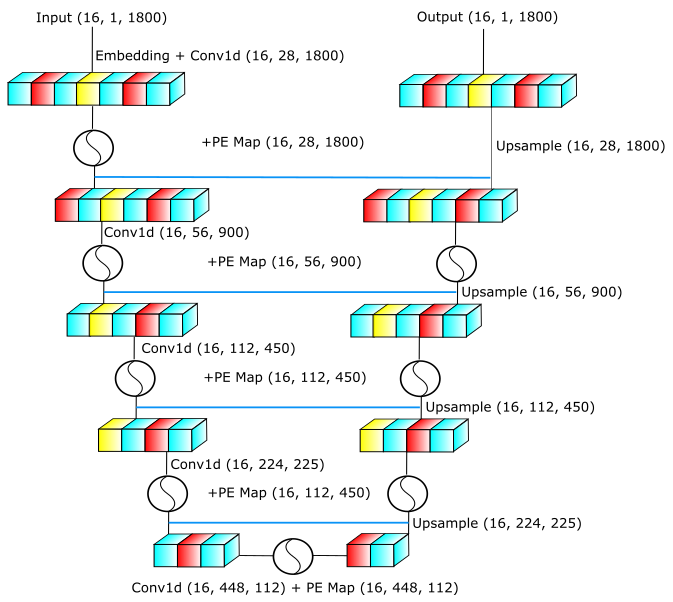
\includegraphics[width=0.7\linewidth]{ch5/figs/unet.png}
    \label{fig:cpunet}
    % \hspace{0.05\linewidth}
    \caption{Schematic diagram of Positional U-Net~(PU-Net). The blue line represents the contracting path. Positional encoding maps at the same level are of the same shape. }
   \label{fig:network_schematic}
\end{figure}

%Unlike Reference~\cite{VAE}, we did not use  Kullback-Leibler Divergence to regulate the reparameterized random distribution.


\subsection{Positional U-Net}
We choose a 1D U-Net~\cite{UNet} as the baseline model when designing the ATN. Positional U-Net contains $n$ convolutional layers to encode each pulse into a feature vector, then uses $n$ upsample layers to decode the feature vector back to an output with the same length. In addition, $n$ contracting paths are established between each pair of convolutional layers and upsample layer at the same level. This network structure allows information at different levels to flow to the decoding part, providing maximal reconstruction efficiency. The Positional U-Net structure is depicted in the left-side panel of Figure~\ref{fig:network_schematic}, where the tensor shape at each stage is also denoted. The Conv1d module in Figure~\ref{fig:network_schematic} is in fact a series of layers, as shown in the left-side panel of Figure~\ref{fig:detail_network}. Within this module, the kernel size is an important hyperparameter to control the reception field of CNN layers, and the padding is added to guarantee the same input and output shape. Max pooling is used in all Conv1d modules but the first one to increase the reception field. 
\begin{figure}[htb!]
    \centering
    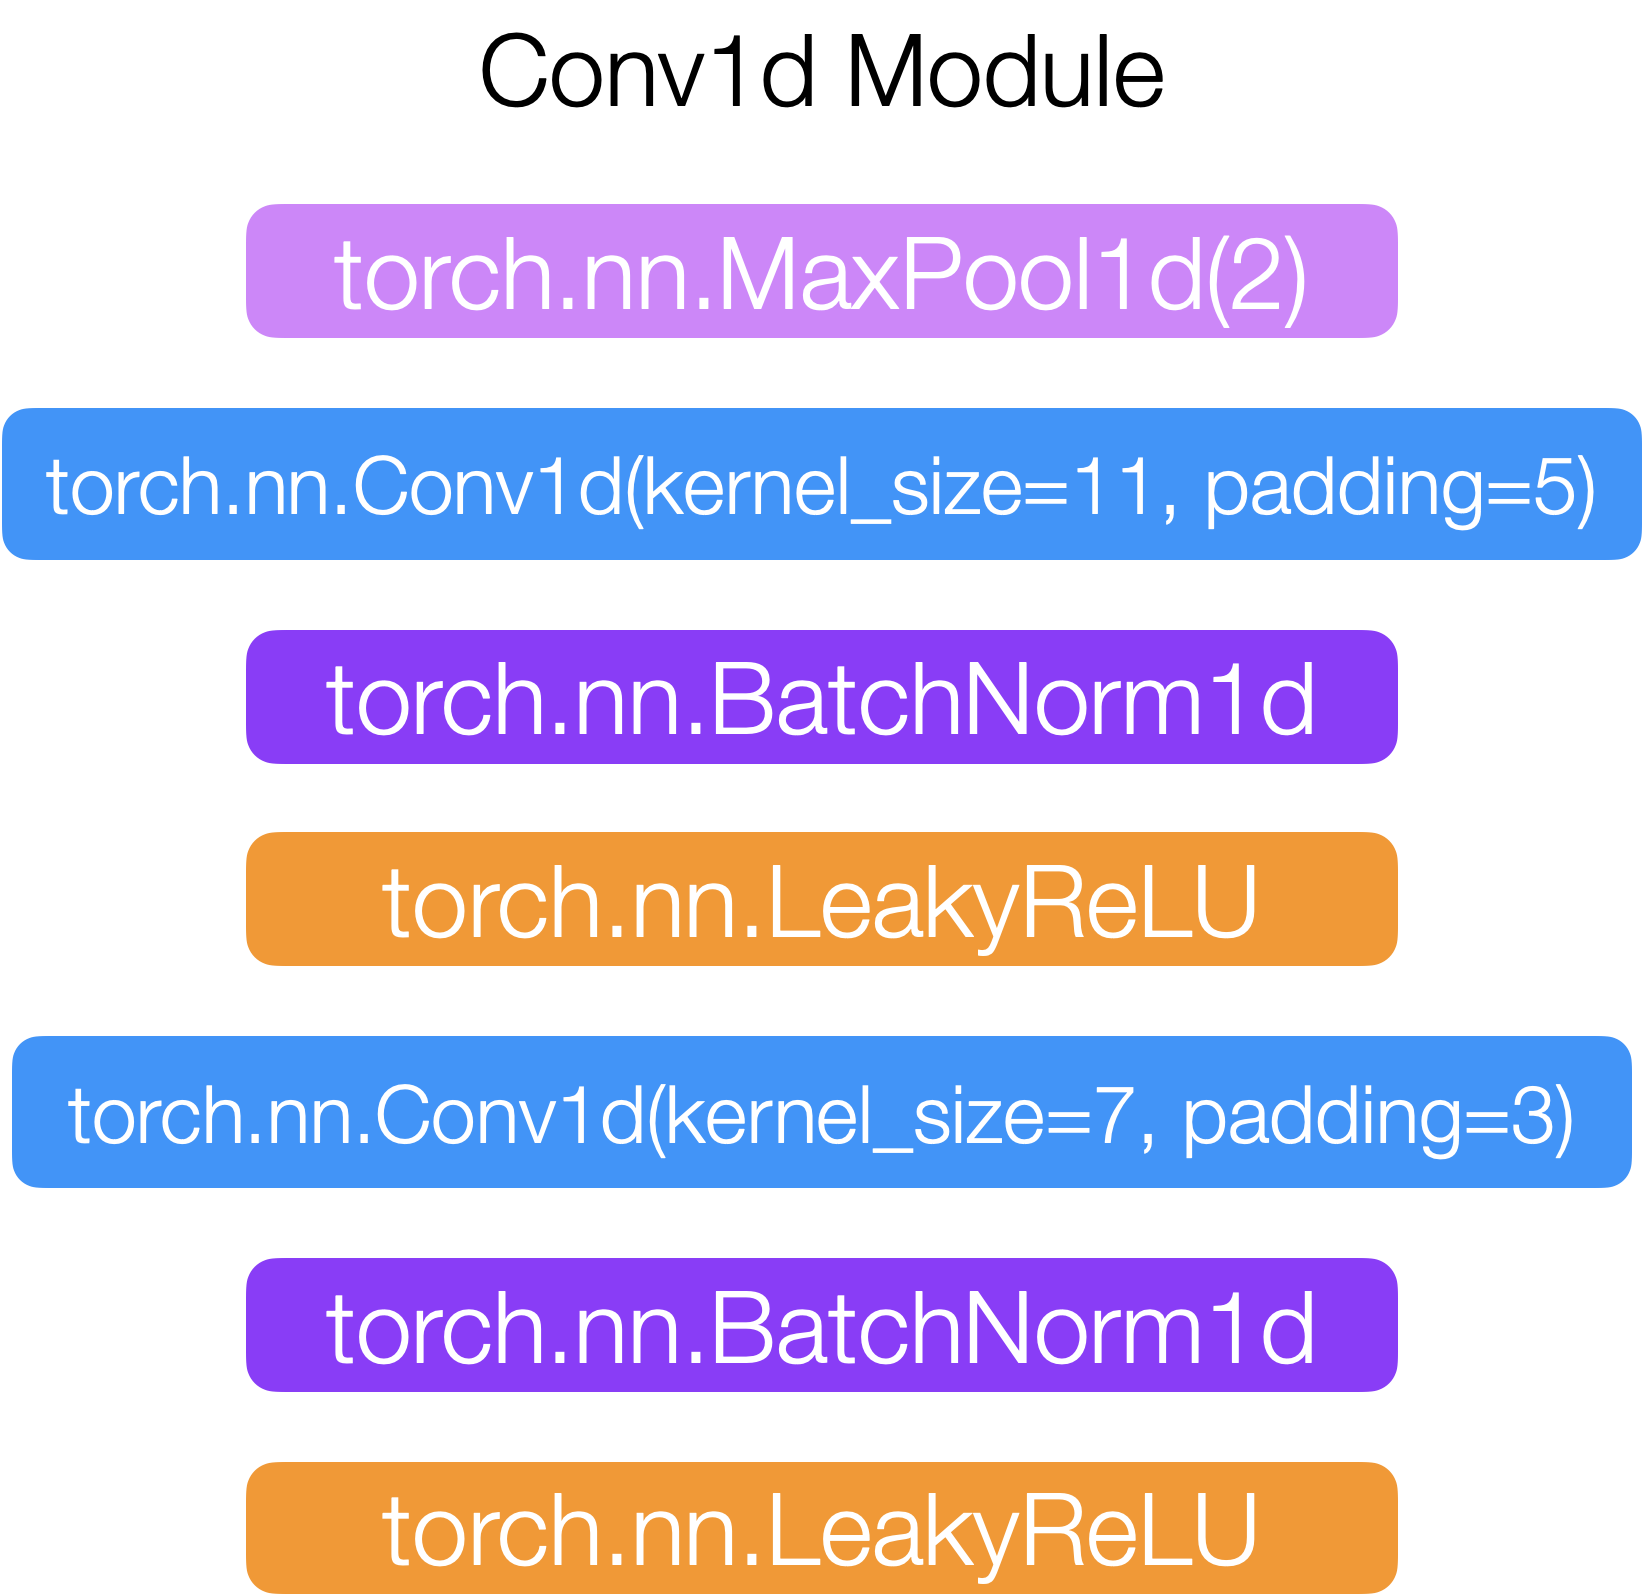
\includegraphics[width=0.3\linewidth,trim={0pc 0pc 0pc 0pc},clip]{ch5/figs/conv1d.png}
    \caption{The layer-wise breakdown of the Conv1d Module in Figure~\ref{fig:network_schematic}.}
    \label{fig:cov1d_break_down}
\end{figure}

During network design, we observed that conventional U-Net does not reproduce the tail of the waveform due to the lack of positional information in intermediate layer outputs. Therefore, we proposed a Positional U-Net~(PU-Net) model with layer-wise positional encoding maps $\mathcal{M}_{\mathrm{position}}$ inspired by the Transformer model~\cite{Transformer}. $\mathcal{M}_{\mathrm{position}}$ contains sine and cosine functions with different frequencies. Since each U-Net layer outputs a tensor with a different shape, $\mathcal{M}_{\mathrm{position}}$ must be generated separately for each layer and added to the layer output, as shown in the left panel of Figure~\ref{fig:network_schematic}. 

PU-Net's layer-wise positional encoding map $\mathcal{M}_{\mathrm{position}}$ is inspired by Reference~\cite{Transformer}. The output of 1D convolutional layer has the shape of $(\mathrm{Batch},\mathcal{d}_{\mathcal{ch}}, \mathcal{d}_{\mathcal{seq}})$, where $\mathcal{d}_{\mathcal{seq}}$ is the length of output feature vector and $\mathcal{d}_{\mathcal{ch}}$ is the number of channels. $\mathcal{M}_{\mathrm{position}}$ is repeated along the batch dimension and then added to the outputs of each convolutional layer and the inputs of each upsample layer. Since those input and output tensors have different $\mathcal{d}_{\mathcal{ch}}$ and $\mathcal{d}_{\mathcal{seq}}$, $\mathcal{M}_{\mathrm{position}}$ has to be generated separately each time.
\begin{equation}
\mathcal{M}_{\mathrm{position}}=
\begin{pmatrix}
\sin(\frac{0}{10000^{0/\mathcal{d}_{\mathcal{ch}}}}) &\sin(\frac{1}{10000^{0/\mathcal{d}_{\mathcal{ch}}}})& \cdots & \sin(\frac{\mathcal{d}_{\mathcal{seq}}}{10000^{0/\mathcal{d}_{\mathcal{ch}}}}) \\
\cos(\frac{0}{10000^{1/\mathcal{d}_{\mathcal{ch}}}}) &\cos(\frac{1}{10000^{1/\mathcal{d}_{\mathcal{ch}}}})& \cdots & \cos(\frac{\mathcal{d}_{\mathcal{seq}}}{10000^{1/\mathcal{d}_{\mathcal{ch}}}}) \\
\sin(\frac{0}{10000^{2 /\mathcal{d}_{\mathcal{ch}}}}) &\sin(\frac{1}{10000^{2/\mathcal{d}_{\mathcal{ch}}}})& \cdots & \sin(\frac{\mathcal{d}_{\mathcal{seq}}}{10000^{2/\mathcal{d}_{\mathcal{ch}}}}) \\
\vdots&\vdots&\ddots&\vdots\\
\cos(\frac{0}{10000^{\mathcal{d}_{\mathcal{ch}}/\mathcal{d}_{\mathcal{ch}}}}) &\cos(\frac{1}{10000^{\mathcal{d}_{\mathcal{ch}}/\mathcal{d}_{\mathcal{ch}}}})& \cdots & \cos(\frac{\mathcal{d}_{\mathcal{seq}}}{10000^{\mathcal{d}_{\mathcal{ch}}/\mathcal{d}_{\mathcal{ch}}}}) \\
\end{pmatrix}
\label{eqn:pos_encoding}
\end{equation}

Lastly, a reparameterization trick is added to the bottom of PU-Net. The trick was proposed by the Variational Autoencoder paper~\cite{VAE} to sample from random space while preserving the gradient flow. Reference~\cite{AAE} pointed out that this trick has the ability to increase the stochasticity of machine learning models. Based on our experimental outcomes, an increased stochasticity helps the ATN and IATN to learn the reconstruction parameters' distributions better. Therefore, we decided to add this method to the latent space vector of PU-Net. Unlike Reference~\cite{VAE}, we did not use  Kullback-Leibler Divergence to regulate the reparameterized random distribution.



\subsection{RNN Discriminator}~\label{subapp:RNN}

We choose attention-coupled recurrent neural network (RNN)\cite{attention} as the discriminator model because position is intrinsically enforced by RNN. A single-layer bidirectional RNN is used as the discriminator model in CPU-Net. We adopt the Gated Recurrent Unit~\cite{GRU} as the internal structure of the RNN. The input raw pulses are first embedded with $m=128$, and the RNN yields a 64-dimensional output $\vec{I}(t)$ at each intermediate step $t$ as well as a final output  $\vec{F}$. We then use an attention mechanism~\cite{attention} to boost the performance of RNN discriminator. The attention mechanism contains an attention matrix A of dimension (64,64), which is used to calculate the attention score between $\vec{F}$ and each $\vec{I}(t)$:
\begin{equation}
    s(t) = \mathrm{Softmax}[\vec{I}(t) A \vec{F}]
\end{equation}
A context vector is produced by summing $\vec{I}(t)$ with the weight $s(t)$ at each $t$. Finally, the context vector and the final output vector are concatenated and fed into a series of fully connected layers to produce a single output. 

\begin{figure}[htb!]
    \centering

    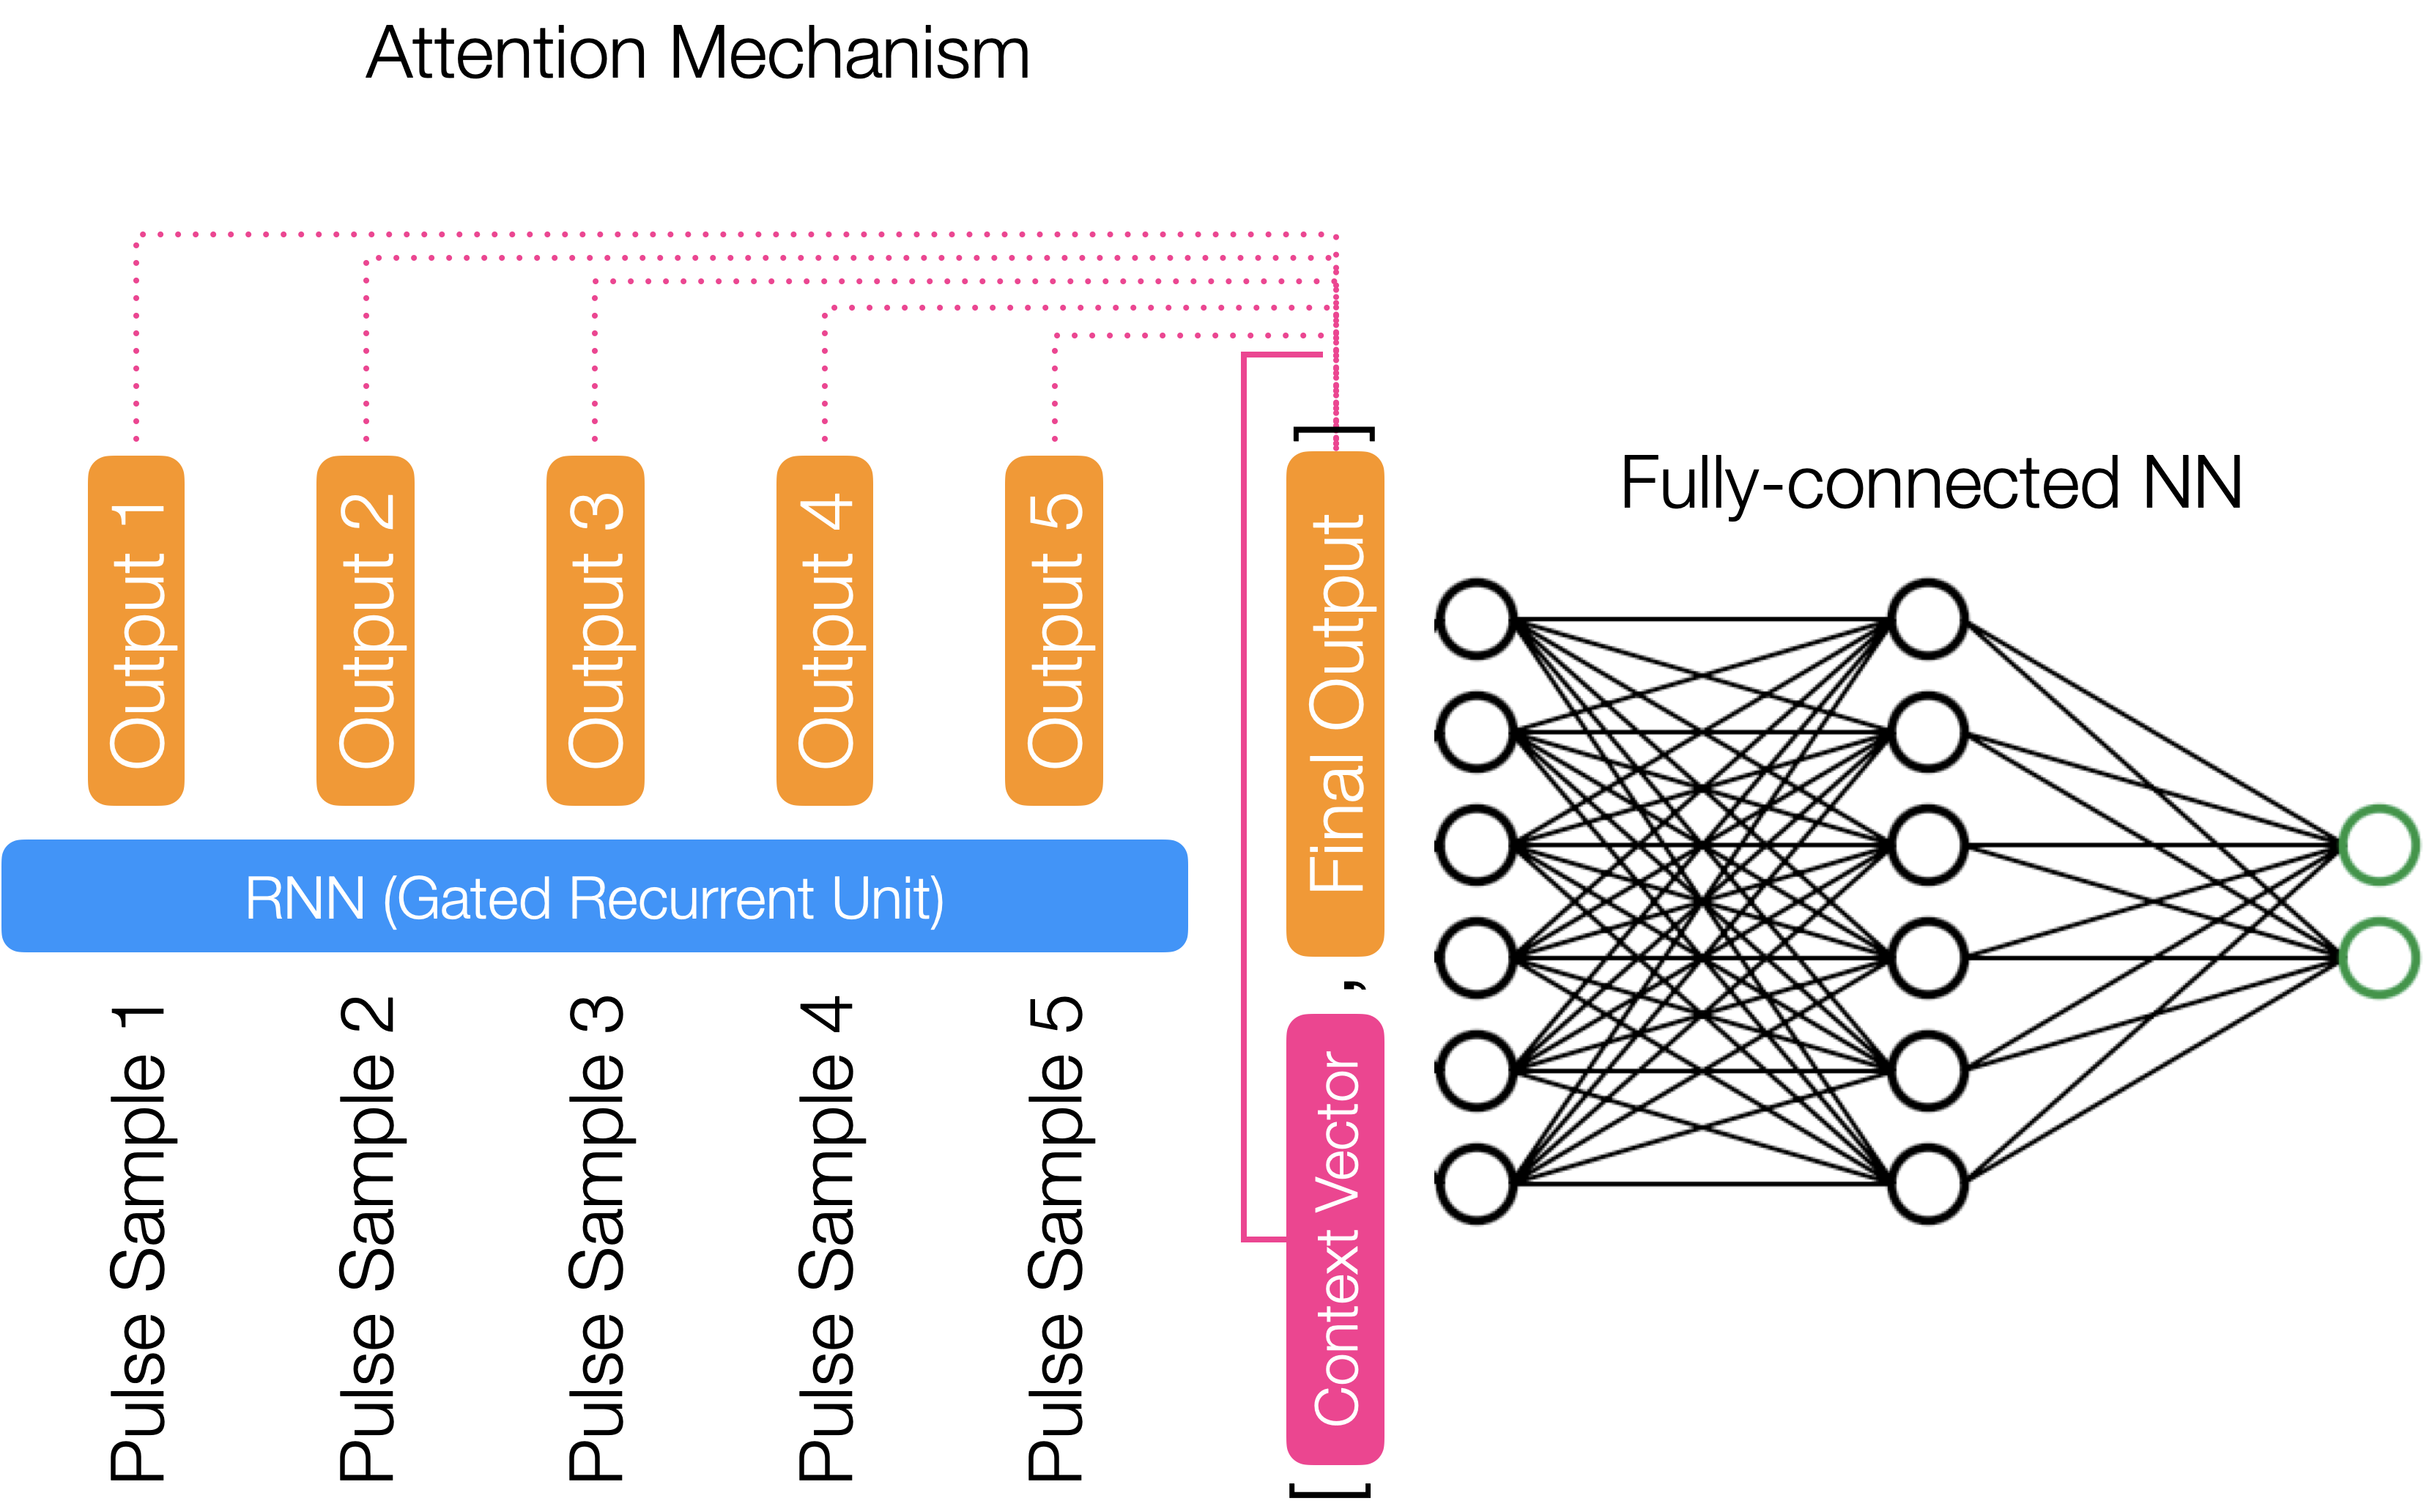
\includegraphics[width=0.7\linewidth,trim={0pc 0pc 0pc 0pc},clip]{ch5/figs/rnnAttention.png}
    \caption{The attention coupled RNN discriminator.}
    \label{fig:detail_network}
\end{figure}



The RNN discriminator is depicted in the right-side panel of Figure~\ref{fig:detail_network}. A single-layer bidirectional RNN is used as the discriminator model in CPU-Net. We adopt the Gated Recurrent Unit~\cite{GRU} as the internal structure of the RNN. The input raw pulses are first embedded with $m=128$, and the RNN yields a 64-dimensional output $\vec{I}(t)$ at each intermediate step $t$ as well as a final output  $\vec{F}$. We then use an attention mechanism~\cite{attention} to boost the performance of RNN discriminator. The attention mechanism contains an attention matrix A of dimension (64,64), which is used to calculate the attention score between $\vec{F}$ and each $\vec{I}(t)$:
\begin{equation}
    s(t) = \mathrm{Softmax}[\vec{I}(t) A \vec{F}]
\end{equation}
A context vector is produced by sum $\vec{I}(t)$ with the weight $s(t)$ at each $t$. Finally, the context vector and the final output vector is concatenated and fed into a series of fully connected layers to produce a single output.




Ideally, the ATN should be trained with paired pulses ($X, X'$) where $Y=Y'$ for each pair. In reality, it is impossible to collect such a paired dataset: we can simulate $\mathcal{T}_{Source}$ from an arbitrary $\mathcal{D}_{Source}$, but it is impossible to collect $\mathcal{T}_{Target}$ so that $\mathcal{D}_{Source} = \mathcal{D}_{Target}$ without knowing the exact form of $P(X'|Y')$. Therefore, the training has to be conducted on $\mathcal{T}_{Source}$ and $\mathcal{T}_{Target}$ given that $\mathcal{D}_{Source} \neq \mathcal{D}_{Target}$. The CycleGAN framework~\cite{CycleGAN} allows us to train ATN on such an unpaired dataset. We first construct two networks an ATN~ $\Lambda$ and an Inverse ATN $\bar{\Lambda}$, both with PU-Net structure. We then construct two discriminator networks $\delta_{S}$ and $\delta_{T}$ for the source and target pulses, respectively. 

Combining all these, we obtain the Cyclic Positional U-Net~(CPU-Net) for Ad-hoc pulse shape simulation. The trained CPU-Net produces both an ATN and an IATN, translating pulses between the source and target domain. The ATN is the primary interest of this work, but the IATN can also be adopted to boost the physical analysis.